%% LyX 2.2.2 created this file.  For more info, see http://www.lyx.org/.
%% Do not edit unless you really know what you are doing.
\documentclass[english,a4paper]{article}
\usepackage[T1]{fontenc}
\usepackage[latin9]{inputenc}
\usepackage{geometry}
\geometry{verbose,tmargin=1.5cm,bmargin=1.5cm,lmargin=2cm,rmargin=2cm}
\pagestyle{empty}
\usepackage{float}
\usepackage{amsmath}
\usepackage{graphicx}
\usepackage{wasysym}

\makeatletter

%%%%%%%%%%%%%%%%%%%%%%%%%%%%%% LyX specific LaTeX commands.
%% Because html converters don't know tabularnewline
\providecommand{\tabularnewline}{\\}
\floatstyle{ruled}
\newfloat{algorithm}{tbp}{loa}
\providecommand{\algorithmname}{Algorithm}
\floatname{algorithm}{\protect\algorithmname}

\makeatother

\usepackage{babel}
\usepackage{listings}
\renewcommand{\lstlistingname}{Listing}

\begin{document}

\title{2ID90 International Draught assignment\\
\emph{template report} }

\author{Group 19: Yoeri Poels, Daan de Graaf}
\maketitle

\section{Introduction}

\emph{Give a short introduction on your project: state the objectives
and comment on how they are achieved. Further more, in the whole document,
please take care of the following:}
\begin{itemize}
\item \emph{Refer to any material you used to obtain your results}, e.g.
\cite{Ertel:2011:IAI:1971988}\emph{.}
\item \emph{Illustrate your material with appropriate figures which are
numbered and have a descriptive caption. Refer to the figure in the
text: see }Figure \ref{fig:The-winners}\emph{.}
\begin{figure}[bh]
\begin{centering}
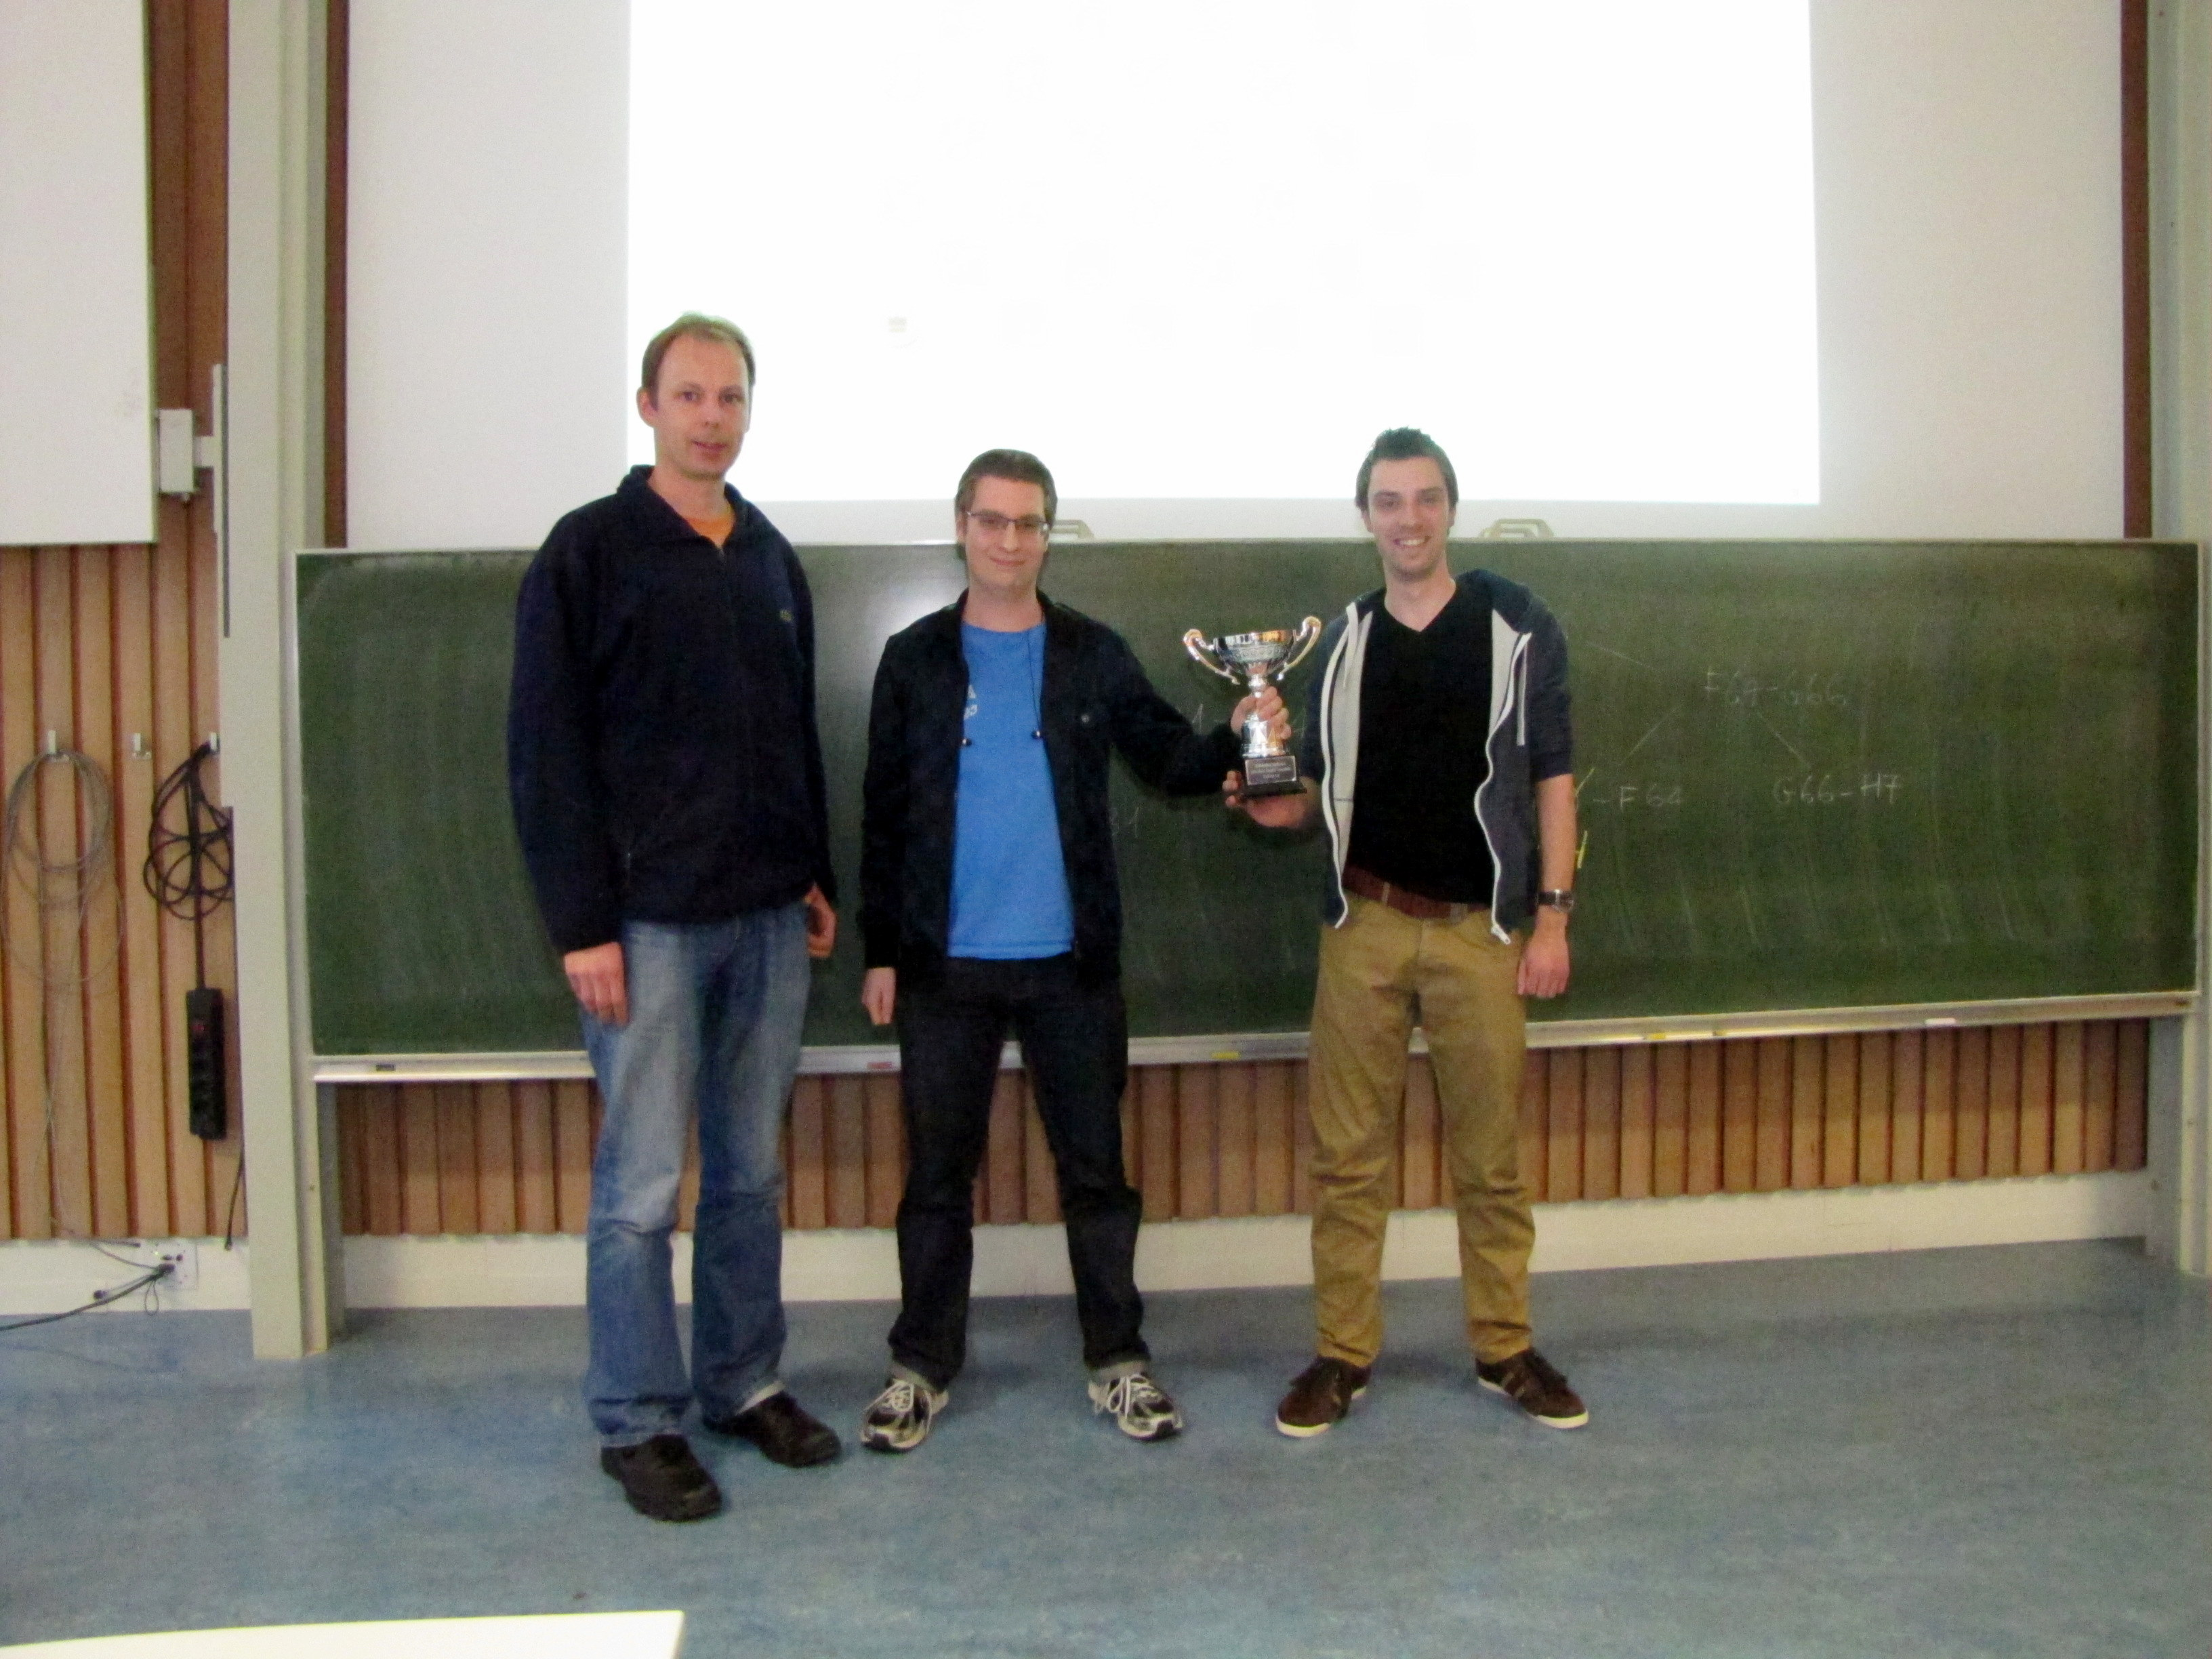
\includegraphics[scale=0.07]{IMG_7778.JPG}
\par\end{centering}
\emph{\caption{\label{fig:The-winners}The winners of the 2ID90 international draughts
tournament, edition 2014.}
}

\end{figure}
\item \emph{Use pseudo-code to explain your algorithms. Note that pseudo-code
is not the same as your actual java code. It should be an abstraction
of that code and should be presented with readability and clarity
in mind. Pseudo-code has to be accompanied with proper explanation
and argumentation.}
\item \emph{Use numbered mathematical formulas instead of lengthy explanations
in text. Additionally, discuss the principles behind the formula.}
\end{itemize}

\section{Alpha-Beta }



\emph{Give a full discussion of how you have implemented and extended
the basic alpha-beta algorithm. Write your algorithms in pseudo-code,
together with proper explanation and argumentation. Don't forget to
refer to them: e.g. see }Algorithm \ref{alg:AlphaBetaMin}\emph{.}

\begin{algorithm}[h]
\begin{lstlisting}[language=Java,numbers=left,numberstyle={\footnotesize},stepnumber=2,basicstyle={\scriptsize},tabsize=4]
int AlphaBetaMin(node, alpha, beta) {
	while (NewNodes not empty)  /* loop over all children of node */
		...
		alpha := Maximum(alpha, Alpha ...) /* recursive call */
		if (alpha >= beta) return beta;
		...	
}
\end{lstlisting}

\caption{\label{alg:AlphaBetaMin}AlphaBetaMin}
\end{algorithm}


\section{Iterative Deepening}

\emph{Give a full discussion of how you have implemented iterative
deepening. Pseudo-code has to be given, as well as a proper explanation
and argumentation for it.}

\section{Evaluation}

\emph{Give a clear explanation of your evaluation function. Compare
alternative evaluation strategies, alternative parameter settings,
etcetera. Argue why you have chosen a particular evaluation function:
make measurements and use graphs and tables where necessary. Use formulas
(like }(\ref{eq:Hs})\emph{) or pseudo-code:
\begin{equation}
H(s)=\begin{cases}
\infty & \fullmoon(s)=0\\
-\infty & \newmoon(s)=0\\
\fullmoon(s)-\newmoon(s) & otherwise
\end{cases},\label{eq:Hs}
\end{equation}
where for board state $s$, $\fullmoon(s)$ and $\newmoon(s)$ are
the number of white and black pieces, respectivily.}

\section{Custom extensions}

\emph{Several extensions for alpha-beta, iterative deepening, and
evaluation exist; for example: move ordering, handling quiescence,
ignoring obliged moves on search depth, and transposition table. Each
implemented extension needs to be clearly documented and its effect
should be proven, e.g. by comparing implementations with and without
the extension using e.g. graphs or tables, featuring, for instance,
'max search depth', and '\#wins'.}

\section{Results}

\emph{If you did not do so already in the previous sections, you can
show your final results here. Again you can use graphs and tables
to show your point.}

\section{Conclusions}

\emph{A short logical summing up of the main reported results.}

\section{Contributions}

\emph{A statement on the contributions of each of the authors.}

\begin{tabular}{|c|c|c|c|}
\cline{2-4} 
\multicolumn{1}{c|}{} & \textbf{implementation} & \textbf{documentation} & \textbf{total \#hours}\tabularnewline
\hline 
Author 1 & 60\% & 30\% & 30\tabularnewline
\hline 
Author 2 & 40\% & 70\% & 25\tabularnewline
\hline 
\end{tabular}
\begin{itemize}
\item \emph{At least the given columns in the table need to be filled in,
add columns if needed.}
\item \emph{Add comments to clarify your table entries when necessary.}
\item \emph{...}
\end{itemize}
\bibliographystyle{plain}
\bibliography{references}

\end{document}
